\section{Erwartetes Ergebnis} 

Unser geplantes Spiellayout sieht vor, dass jeder Client eigentlich nur bis zu 6 seiner eigenen Nachbarn kennt. Der Rest des Spiels ist ihm nicht direkt bekannt. Dadurch wollen wir erreichen, dass der Workload lokal in einer kleinen Gruppe bleibt und sich nicht auf das komplette System exponentiell auswirkt.

\begin{figure}[hbt]
  \centering
  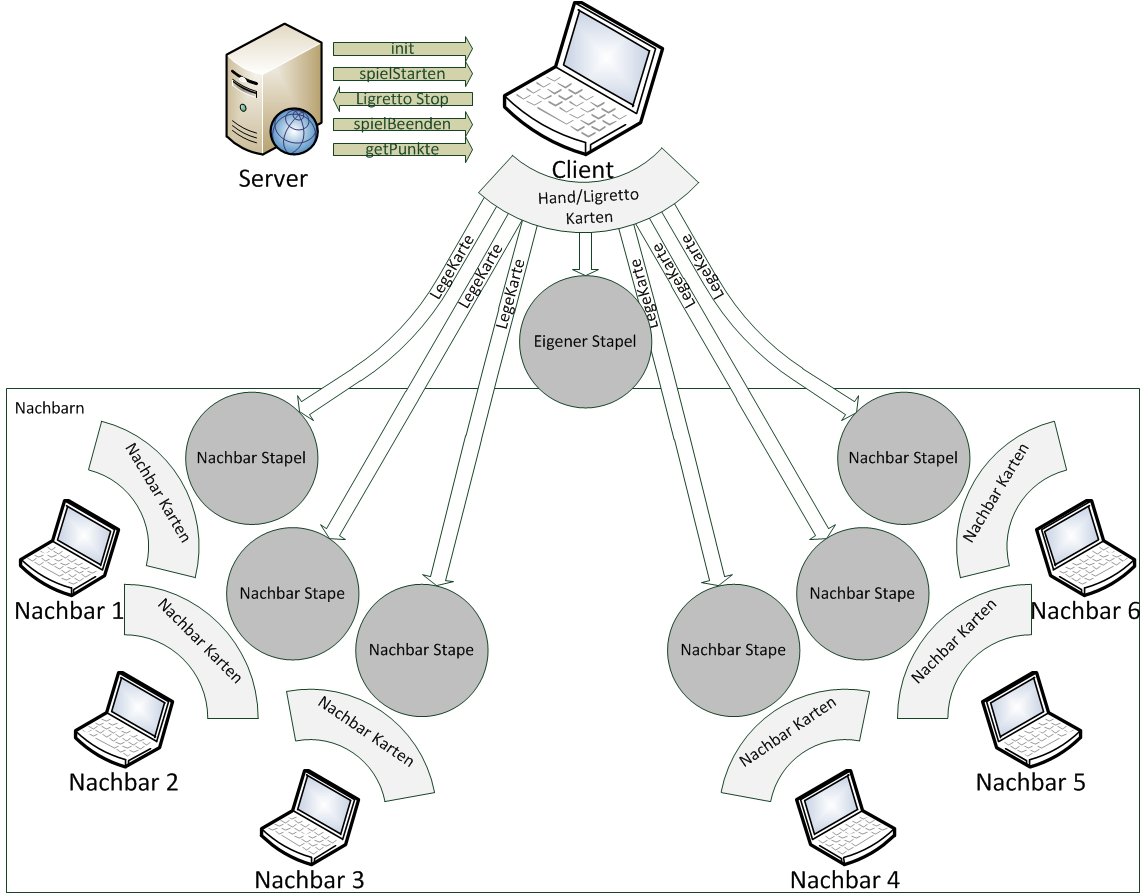
\includegraphics[width=0.9\textwidth,angle=0]{graphics/SpielLayout.png}
  \caption{Spiel aus Client-Sicht \hfill{} }
  \label{ergebnisspiellayout}
\end{figure}

Abbildung~\ref{ergebnisspiellayout} zeigt, wie sich der Client verhält und was er wahrnimmt. Er bekommt vom Server alle nötigen Inputs und versucht, auf den eigenen und den Stapeln seiner Nachbarn seine Karten zu legen. Gelingt ihm dies nicht, geht er weiter zur nächsten Karte, bis es ihm gelingt. 

Wir hatten uns überlegt, zuerst zu prüfen, ob auf einem Nachbar Stapel eine Karte gelegt werden könnte und es dann zu tun, sind aber von diesem Ansatz wieder abgekommen, weil dem aufrufenden Client in der Zwischenzeit sehr wahrscheinlich bereits andere Clients zuvorkommen würden und damit viele Versuche (eine Karte zu legen) sowieso misslingen würden. Ob der Client ständig versucht, eine Karte zu legen oder ob eine Karte legbar ist und danach versucht, die Karte zu legen, kommt fast auf das Selbe hinaus. Wir haben uns aber dafür entschieden, nur die Karten zu legen, da damit die RMI Calls minimiert werden.

Generell hat unsere verteilte Lösung ein Problem, sobald ein beliebiger Client ausfällt. Sollte ein Nachbar ausfallen, so wartet der Client unter Umständen sehr lange auf einen Timeout, bis er weiter machen kann. Vermutlich sind in der Zeit andere Clients bereits mit ihrem Spiel fertig und alle Nachbarn des ausgefallenen Clients währen mit dem Warten auf das Timeout "beschäftigt".

Um dieses Risiko zu vermindern, muss garantiert werden, dass kein Client ausfällt. Ansonsten muss das Spiel nochmals wiederholt werden.



\subsection{Auswirkungen bei starker Skalierung}

Aufgrund unserer geplanten Limitierung des Clients auf seine 6 Nachbarn wird der Workload innerhalb des Spiels linear verteilt. 

Jeder Client hat (egal wie gross das Spiel ist) immer nur maximal 6 Nachbarn, die versuchen, bei ihm Karten auf die Stapel zu legen. Damit erhöht sich der Workload für die Clients nicht, egal wie viele Clients am Spiel teilnehmen.

Der Knackpunkt ist jedoch die Verteilung des Start- und Endsignals.


\subsubsection{Start- und Endsignal ohne Timestamp}

\color{red}
\textbf{WELCHE LÖSUNG WÄHLEN WIR? ICH HABE MAL BEIDE DOKUMENTIERT}
\color{black}

Der grösste Knackpunkt ist die zeitliche Verteilung des \textit{SpielStart} und \textit{SpielBeenden} Signals \textbf{ohne} Timestamps.

In einem 100 Mbit/s LAN  ist die durchschnittliche Latenz bei ca. \unit{60}{\micro\second}.

Dadurch ergibt sich pro Client ein Zeitzuwachs für das Verteilen des \textit{SpielStart} und \textit{SpielBeenden} Signals.

\begin{figure}[hbt]
  \centering
  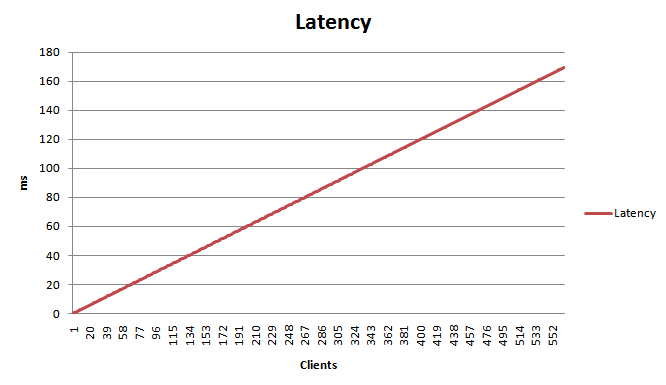
\includegraphics[width=0.9\textwidth,angle=0]{graphics/latency.png}
  \caption{Zeit für das Verteilen des Start- oder Endsignals \hfill{} }
  \label{ergebnislatency}
 \end{figure}
 
Abbildung~\ref{ergebnislatency} zeigt, wie sich die Zeitdauer mit erhöhter Client Anzahl verlängert.
 
\textbf{Problem:}

Jeder Client hat immer 4 Karten die er legen muss plus eine Karte aus seinen Handkarten, die er optional auch noch legen könnte. Er versucht, jede Karte bei 6 Nachbarn zu legen. Wir gehen von einer Fehlerrate von ca. 98\% aus. Das heisst, nur eine aus 50 Karten kann überhaupt gelegt werden. Tendenziell geht diese Fehlerquote sogar eher noch höher.

Im Best Case legt der Gewinner des Spiels genau 10 Karten, im Worst Case legt er 36 Karten. Im Durchschnitt legt der Sieger eines Spiels (reales Spiel mit Karten) ca. 20 Karten. 

\textbf{Best Case:} Um 10 Karten zu legen (bei einer 98\% Fehlerrate) muss der Client 500 Versuche starten, um eine Karte zu legen. \unit{500} * \unit{60}{\micro\second} = \unit{30000}{\micro\second} = \unit{30}{\milli\second}.

\textbf{Average Case:} Um 20 Karten zu legen (bei einer 98\% Fehlerrate) muss der Client 1000 Versuche starten, um eine Karte zu legen. \unit{1000} * \unit{60}{\micro\second} = \unit{60000}{\micro\second} = \unit{60}{\milli\second}.

\textbf{Worst Case:} Um 34 Karten zu legen (bei einer 98\% Fehlerrate) muss der Client 1700 Versuche starten, um eine Karte zu legen. \unit{1700} * \unit{60}{\micro\second} = \unit{102000}{\micro\second} = \unit{102}{\milli\second}.

\textbf{Fazit:}

Bereits ab einer Spielerzahl von ca. 100 Clients hat der erste Spieler im Best-Case bereits gewonnen, bevor der letzte das Startsignal erhält.

Ab einer Spielerzahl von 200 hat bereits im Average-Case der erste Spieler gewonnen, ab einer Spielerzahl von 350 tritt sogar der Worst-Case ein.

Man kann also sagen, dass das Spielresultat voraussichtlich nur bis etwa 10 Spieler einigermassen zufällig ist. Von 10 bis 50 ist der Vorteil bereits klar bei den ersten 10 Spielern; alle Spieler von 50-100 haben keine reale Chance mehr zu gewinnen, da der Gewinner sicher unter den ersten 50 sein wird. 

\subsubsection{Start- und Endsignal als Timestamp}

\color{red}
\textbf{DIES WÄR DIE ALTERNATIVE LÖSUNG}
\color{black}

Werden Timestamps benutzt, um die Start- und Endsignale zu übertragen, stellt dies zwar grössere Anforderungen an die Zeitsynchronisation und die KI, aber die Möglichkeit, dass ein Client gewinnt, ist dabei absolut zufällig.

Der erste Knackpunkt ist die Verteilung der Karten sowie das Startsignal. Der Server benötigt eine gewisse Zeit, um die Karten zu verteilen. Anschliessend benötigt er eine gewisse Zeit, allen Teilnehmern das Startsignal zu übermitteln. Um sicherzustellen, dass alle zur gleichen Zeit starten, haben wir uns entschieden, das Startsignal in Form eines Startzeitpunkts ein paar Sekunden in der Zukunft zu definieren. Damit kann sichergestellt werden, dass alle Clients exakt zum gleichen Zeitpunkt mit dem Spiel starten können.


Der zweite Knackpunkt in unserem System mit sehr vielen Clients ist der Zeitpunkt, zu dem ein Client \textit{Ligretto-Stop!} aufruft. In diesem Augenblick muss der Server bei allen Clients das Spiel beenden. Dies kann bei sehr vielen Clients eine gewisse Zeit dauern, bis alle Clients das Stopsignal bekommen haben. Da wir aber mit einem Timestamp sicherstellen, dass das Stopsignal auch rückwirkend gültig ist, ist auch dies kein Problem. Es stellt aber erweiterte Anforderungen an die KI, ihre Schritte rückgängig zu machen, sollte das Stopsignal erst einige Zeit nach dem eigentlichen Stopzeitpunkt ankommen.

Der dritte (jedoch unkritische) Knackpunkt ist das Abholen der Punkte. Der Server hat dafür jedoch keinen Zeitdruck, da alle Clients bereits gestoppt sind. Es kann aber eine gewisse Zeit dauern, bis alle Clients ihre Punkte abgegeben haben, da der Server jeden einzelnen anfragen muss.


%Ausarbeitung / Darstellung (0 Punkte / max. 2 Bonuspunkte)
%    - Grafiken Zusatzpunkte erhalten Sie hier für eine gute Ausarbeitung wie spezifische Grafiken / Ablaufdiagramme etc. max. 2 Punkte. 0 Punkte ist 'normal', 1/2 Punkt für 1-2 spezifische nutzbringende Grafiken, 1 Punkte für ausführliches Nutzen von Grafiken.
%    - Detaillierungsgrad: Je nach Tiefe und Detaillierungsgrad Ihrer Ausarbeitung können Sie bis zu einem Zusatzpunkt holen (0=normal, 1/2=detailliert, 1=sehr detailliert)